\section{Architektura informacji}
\subsection{Schemat bazy danych}
\begin{figure}[h]
    \centering
    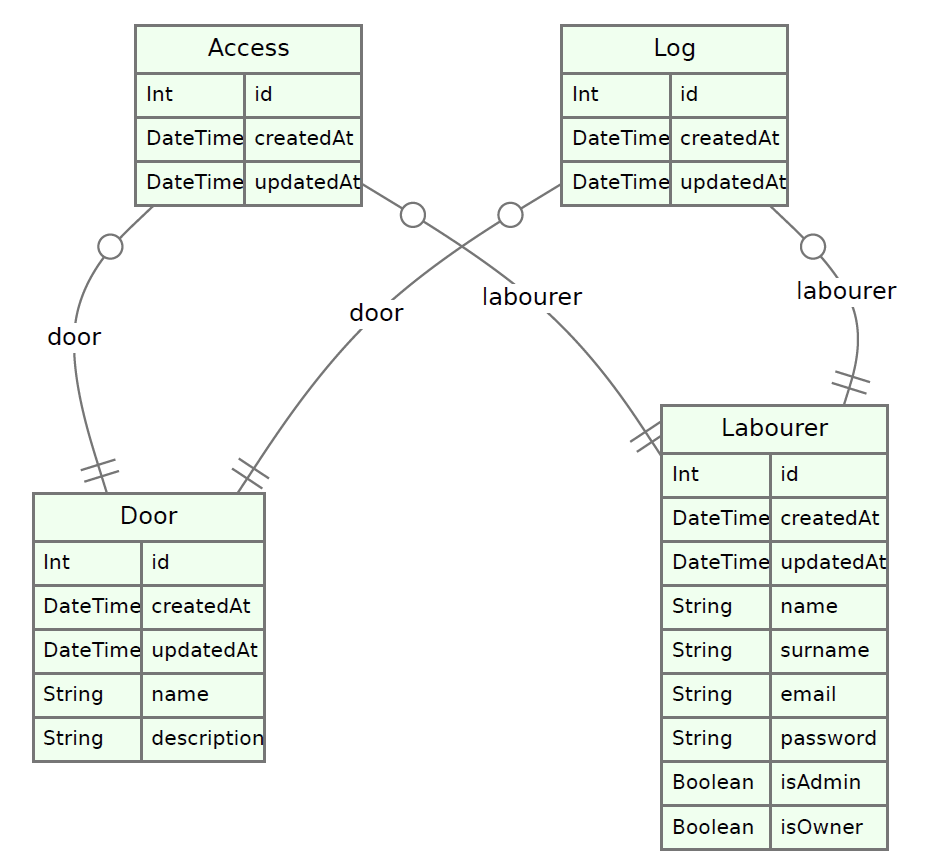
\includegraphics[scale=0.6]{photos/schemat_bazy_danych.png}
    \caption{Schemat bazy danych}
    \label{fig:erd}
\end{figure}
\newpage
\subsection{Stworzenie bazy danych}



\subsection{Opis encji w bazie dancyh}

\subsubsection{Tabela Labourers}
\noindent Tabela zawierająca wszystkie informacje dotyczących użytjowników aplikacji - są w 
w niej zawarte informacje o użytkownikach, którzy są pracownikami, 
administratorami i właścicielami.
\begin{table}[h]
    \centering
    \scalebox{0.75}{
    \begin{tabular}{|c|c|c|c|c|c|c|c|c|}
    \hline
    \textbf{id} & \textbf{createdAt} & \textbf{updatedAt} & \textbf{name} & \textbf{surname} & \textbf{email} & \textbf{passowrd} & \textbf{isAdmin} & \textbf{isOwner} \\ \hline
    int AI PK   & datetime(3)        & datetime(3)        & varchar(191)  & varchar(191)     & varchar(191)   & varchar(191)      & tinyint(1)       & tinyint(1)       \\ \hline
    \end{tabular}}
    \caption{Tabela Labourers}
    \end{table}


\subsubsection{Tabela Door}
\noindent Tabela zawierająca wszystkie informacje dotyczące drzwi -
 są w niej zawarte informacje: kiedy zostały stworzone, kiedy zostały ostatnio do kogoś przypisane, 
 nazwa oraz opis drzwi.
 \begin{table}[h]
    \centering
    \scalebox{0.75}{
    \begin{tabular}{|c|c|c|c|c|}
    \hline
    \textbf{id} & \textbf{createdAt} & \textbf{updatedAt} & \textbf{name} & \textbf{description} \\ \hline
    int AI PK   & datetime(3)        & datetime(3)        & varchar(191)  & varchar(191)         \\ \hline
    \end{tabular}}
    \caption{Tabela Door}
\end{table}

\subsubsection{Tabela Access}
\noindent Tabela zawierająca wszystkie informacje dotyczące uprawnień do drzwi-
są zawarte w niej informacje: kiedy zostały stworzone, kiedy zostały ostatnio zmodyfikowane,
jakie drzwi są do jakiego użytkownika przypisane.
\begin{table}[h]
    \centering
    \scalebox{0.75}{
    \begin{tabular}{|c|c|c|c|c|}
    \hline
    \textbf{id} & \textbf{createdAt} & \textbf{updatedAt} & \textbf{doorID} & \textbf{labourerID} \\ \hline
    int AI PK   & datetime(3)        & datetime(3)        & int           & int               \\ \hline
    \end{tabular}}
    \caption{Tabela Access}
\end{table}

% \subsubsection{Tabela AccessAddedByLog}
% \noindent Tabela zawierająca wszystkie informacje dotyczące logów dodawania uprawnień do drzwi - SA
% są w niej zawarte informacje: kiedy zostały stworzone, kiedy zostały ostatnio zmodyfikowane, 
% indetyfikator dostępu, identyfikator administratora, identyfikator drzwi, do których zostały dodane uprawnienia.
% \begin{table}[h]
%     \centering
%     \scalebox{0.8}{
%     \begin{tabular}{|c|c|c|c|c|c|}
%     \hline
%     \textbf{id} & \textbf{createdAt} & \textbf{updatedAt} & \textbf{accessID} & \textbf{adminID} & \textbf{doorID} \\ \hline
%     int AI PK   & datetime(3)        & datetime(3)        & int             & int           & int              \\ \hline
%     \end{tabular}}
%     \caption{Tabela AccessAddedByLog}
% \end{table}


% \subsubsection{Tabela DoorOpenedLog}

% \noindent Tabela zawierająca wszystkie informacje dotyczące logów otwierania drzwi - 
% są w niej zawarte informacje: kiedy zostały stworzone, 
% kiedy zostały ostatnio zmodyfikowane, identyfikator drzwi
% oraz identyfikator użytkownika.  
% \begin{table}[h]
%     \centering
%     \scalebox{0.8}{
%     \begin{tabular}{|c|c|c|c|c|}
%     \hline
%     \textbf{id} & \textbf{createdAt} & \textbf{updatedAt} & \textbf{doorID} & \textbf{labourerID} \\ \hline
%     int AI PK   & datetime(3)        & datetime(3)        & int           & int               \\ \hline
%     \end{tabular}}
%     \caption{Tabela DoorOpenedLog}
% \end{table}

